\documentclass[]{report}
\renewcommand{\thesection}{\arabic{section}}
\usepackage{graphicx}
% Title Page
\title{Implementing neural networks with tensorflow report}
\author{Linus Edelkott, Tobias Petri}


\begin{document}
\maketitle

\begin{abstract}
The aim of this project is to create a virtual Texas Hold'em player by using a convolutional neural network, based on the paper "Poker-CNN: a pattern learning strategy for making draws and bets in poker games" \cite{1} by Yakovenko, Nikolai et. al.
The aim is to imitate human poker-playing behaviour, including bluffing, as close as possible - a task where current, non neural network based poker bots usually fail.
\end{abstract}


\section{Introduction}
Unlike other games such as chess or checkers, poker provides an especially challenging task for computer players (bots). That is because poker contains a very "human" component aside from its set of rules: the bidding, raising, the bluffing. Where other games only provide a reward upon successfully winning them, the reward itself is a key element of the poker turn structure. Furthermore, since Texas Hold'em poker can be played with up to 9 people at a regular game, the state space grows to an enormous size. All these factors lead to the fact that current bot implementations usually are rather weak. Confronted with a human player, these bots have the huge disadvantage of being predictable: They often show repetitive behaviour and are bad at bluffing. Self learning systems though can put an end to this, as the Libratus project shows\cite{2}: Developed at the Carnegie Mellon University, Libratus was able to beat 4 pro poker players in a 20 day tournament. After initially losing, the bot changed its strategy after day 4. Analogous to Libratus, the team of Yakovenko, Nikolai et. al. developed a CNN based approach that aims at surpassing the current implementations and being competitive with human tournament players \cite{1}. As their data source, they used simple bots to generate a large training and validation set. Learning only from the successful games, the CNN should afterwards be easily able to surpass the weak bots.    

\section{Poker-CNN: A Pattern Learning Strategy for Making Draws and Bets in Poker Games}
\subsection{The original paper}

In the paper ``A Pattern Learning Strategy for Making Draws and Bets
in Poker Games''\cite{1} the authors propose a convolutional neural
network, which should be adaptable for all poker variants under the
hypothesize that poker games can be described as a pattern matching
problem. The poker network learns through iterative self-play and
improves using the results of its previous actions for training. The
main challenges for a data driven approach like this one, is to find
a good representation of the game (which can be adapted to several
poker games) and to arrive at a sophisticated result using self-generated,
imperfect data.

In order to solve the first challenge, the authors introduce a unified
representation of poker games. To encode the game state into a form
which can be used in a convolutional network the game information
is described in different matrices. There are 13 ranks of poker\footnote{2,3,4, ..., J,Q,K,A}
cards and 4 different suits\footnote{club, diamond, heart, spade},
so each card is represented in a 4 x 13 sparse binary matrix, where
only one element is non zero. To capture the full hand information
a further layer is added, the sum of the previous layers. The advantages
in doing so are: a large input builds a good base for a CNN and the
full hand representations makes it easier to model common poker patterns,
``without game specific card sorting or suit isomorphisms (e.g. AsKd
is essentially the same as KhAc)''.\cite{1} Because poker is not
only expressed in cards, context information need to be passed to
the CNN as well. For example the number of chips in the pot is represented
as a numerical coded 4x13 matrix, where the minmal amount is coded
similar to the smallest poker card and the maximal amount\footnote{4{*}13{*}minimal amount (small blind), everything higher than this
is encoded identical} is encoded as a binary matrix (entails only ones). A binary 4x13
matrix (two-player games) is used to represent the position, hence
it entails whether the system is first to bet. Further layers are
added, which are not relevant for Texas Hold'em. Each matrix is finally
zero padded to a 17x17 matrix to ease the convolutions and max pooling.
The whole Yx17x17 tensor is used as input. In section \ref{see:adapted_p}
we discuss our extended representation for Texas Hold'em no Limit
Cash Game.

Different poker games usually consist of either betting or draw actions,
in rare cases there are both type of actions. 

Draw actions are defined as actions in which the player has the option
to replace one or more of his cards with a new drawn card. The task
for a neural network concerning draws is to estimate the return of
every possible card replacement and select the one with the highest
output. Yakovenko, Nikolai et. al. employed Monte Carlo Sampling to
first generate 250000 poker hands and simulate the expected outcome
for each possible draw, for each of these hands.

While the 250000 hands are encoded into the input tensor, the expected
outcome will serve as label. The authors did train three different
networks: a fully connected neural network, a convolutional layer
with a filter size of 5x5 and a convolutional neural network with
the filter size of 3x3. The latter one outperformed the other two,
hence we used this one as basis. Further details of the network will
be discussed in section \ref{see:CNN_arc}. 

Betting actions on the other hand are defined as action in which the
player evaluates the win chance of his current hand and places a corresponding
amount of chips. If he sees no winning chance at all he can quit the
round in which he also loses his already placed bets. Important to
notice is that players don't has to be honest about his hand and may
raise (bet a higher amount of chips than the previous players) regardless
in order to bluff the other players into folding. Due to this fact
there is often not ``one'' right move. Players often vary their
actions although their cards might be similar. 

In the case of Texas Hold'em limited Poker, which was used in the
paper as trainings example, the player has 5 betting actions:

Check - bet nothing, but keep playing), which is only possible if
their are no bets in this round so far

Bet - start to actually put something in the pot

Raise - set a higher amount of chips than the previous players

Call - match the bet of the previous players

Fold - give up the current hand

Due to this different options the expected outcome can not simply
be estimated by Monte Carlo sampling. Thus for each training hand
several epochs of this hand were simulated using simple heuristic
bots, which adjusted their winning chance according to the previously
simulated allin probabilities. Once again the expected outcome of
this simulation was used as label for the respective hand. Overall
500000 hands were used for training. 

As a result the CNN was finally able to outperform the bot used for
training and was even competetive against a human expert.

\subsection{Input adaption for (regular) Texas Hold'em \label{see:adapted_p} }

Texas Hold'em Poker is one of the most popular poker variants existing
and hence we wanted to examine how the CNN would be able to perform
when trained on it. In fact Yakovenko, Nikolai et. al. already implemented
Texas Hold'em as training data set, but they used a simplified version.

Our initial goal was to implement the CNN on training data containing
the game states of (regular) ``9 player Texas Hold'em no Limit (cash-game)''.
The main difference hereby aside from the player count is that in
limited poker the player may only bet and raise a fixed amount.

In general Texas Hold'em consists of 4 betting rounds. At first each
player gets 2 cards, known as hole cards and the first betting round
begins. Afterwards 3 community cards (the flop) are drawn which are
visible for everyone and constitute the current hand of each player
together with their respective hole cards. The next betting round
starts and the game continues with the drawing of a single community
card and the following betting round which will be repeated once more
(the turn and river). The 5 best cards out of this 7 constitutute
the hand of each player and determines the winner.

Instead of using a 4x13 matrix for each indivudal card we used one
matrix for each round. Thus the first 4x13 matrix has two elements
different than zero, the second one has 3 and the others have one,
respectively. Hence the network shouldn't differentiate between the
sequence of cards entailed in one round (e.g. 5s5c is identically
to 5c5s). The layer containing all cards information (the sum of the
previous 7) will be kept. Furthermore using one binary matrix as input
is no longer sufficient. A 9x9 matrix will be used instead, where
each row despite one will be zero. The row filled with ones marks
the position (who is first to bet). Another 9x9 matrix entails information
about the state of the other players, if the respective row is 1 they
are still active and didn't fold yet. Additional to the numerical
coded amount of chips in the pot a second similarly coded matrix containing
the amount of chips placed in the current betting round is needed.
We assume that a really competetive Player would need more information
but assumed that this would increase the learning phase. The final
representation is a 9x17x17 tensor, summarized in Table \ref{tab:tensor}.
%\begin{figure}[h]
%	\begin{table}
	%	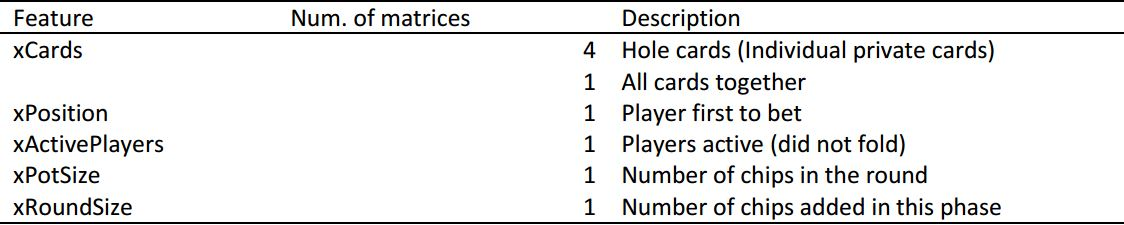
\includegraphics[scale=0.5]{Features.JPG}
%		\caption{Features used as inputs for Texas Hold'em no Limit Poker \label{tab:tensor}}
%	\end{table}
%\end{figure}

\section{The CNN architecture \label{see:CNN_arc} }

The convolutional neural network that was used within this project has an architecture similar to the original CNN from the paper\cite{1}. While Yakovenko, Nikolai et. al. compared a fully connected network, a CNN with 3x3 filters and a 5x5 filter CNN, We decided to only compare 3x3 and 5x5 CNNs. Using Tensorflow gave us the advantage of using 3d convolution, unlike the 2d convolution used in the original network\footnote{The paper does not specify the exact type of convolution used. However, based on the github projects of the author, we assume 2d convolution.}. With the input as explained in section 2.2, the first two layers are 3d convolutional, with a max pool after the second. This is followed by yet another 2 convolutional layers with max pool, only with decreased size. 
Afterwards, a dense 50\% dropout layer feeds directly into the output layer. Figure 1 shows the network structure from the paper. Aside from the different input, the output of our implementation has also been modified: Where the original had 5 output neurons, our version has only 2, representing the options 'fold' and 'call'. These are the only relevant moves, since our training opponent is an allin bot.


\begin{figure}[h]
	\caption{Network structure}
	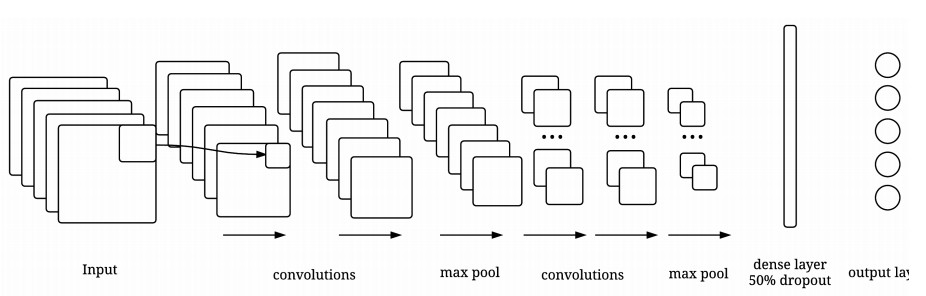
\includegraphics[scale = 0.5]{cnn_structure.jpg}
\end{figure}

The network was trained using a dataset generated by PyPokerEngine. A heuristic player played continuously, while only the games where it also won were kept. The enemy of this heuristic player was an allin bot, which leaves the player two choices: Fold or call. While we initially started out with a 10 label dataset to represent all possible actions the player could perform, we decided to reduce it two 2 because this reduces the overall complexity and because more possible actions are simply not necessary for our scenario. Also, the initial CNN struggled with the 10 label format and mostly produced bad results which made the label reduction a necessary step

The dataset that was used to train our final version contained 65000 samples. 

\section{Evaluation \label{see:evaluation} }

Unfortunately we were not able to produce any significant results and our network was unable to learn how to beat even a simple Allin bot. In order to find the source of error we tried several different settings. However it didn't make a difference if the used kernel were 5, 16 or 32, neither did it make a difference whether we used the whole tensor as input, or only the hole cards. We assume that this is caused by varying reasons. 

First of all, even 65000 hands are probably not enough to train the if we compare it to the 2598960 possible hole cards in Poker. However even when run on the same hands repeatedly (several epochs) the network did not suceed in classifying a winning move.

\begin{thebibliography}{}
	\bibitem{1} Yakovenko, Nikolai, et al., \emph{Poker-CNN: a pattern learning strategy for making draws and bets in poker games.}, arXiv preprint arXiv:1509.06731 (2015).
	
	\bibitem{2} Rivercasino.com, \emph{Brain VS AI},
	riverscasino.com/pittsburgh/BrainsVsAI

\end{thebibliography}  



\end{document}  
